\documentclass[a4paper,14pt]{extreport}
\usepackage[utf8]{inputenc}
\usepackage[T2A]{fontenc}
\usepackage[russian]{babel}
\usepackage{eufrak}
% поля:
\usepackage[left=1cm, right=1cm, top=2cm, bottom=2cm]{geometry}
\linespread{1}
\usepackage{indentfirst} % отделять первую строку раздела абзацным отступом
\setlength\parindent{5ex}
\addto{\captionsrussian}{\renewcommand*{\contentsname}{Содержание}}
\usepackage[hidelinks]{hyperref} % гиперссылки в содержании
\usepackage{graphicx}
\usepackage{float}
\usepackage{amsmath}
\renewcommand*{\thesection}{\arabic{section}}

\usepackage{multirow}
\usepackage[normalem]{ulem}
\useunder{\uline}{\ul}{}

\usepackage{cmap}%позволяет копировать кириллицу из скомпилированного файла

% Глубина разделов, попадающих в содержание
\setcounter{tocdepth}{3}

\linespread{1.3} % настройка межстрочного интервала
\tolerance=1000 % настройка чувствительности вставки переносов
\hfuzz=0pt
\sloppy

\begin{document}
	
	\begin{titlepage}
		\begin{center}
			\large
			МИНИСТЕРСТВО ОБРАЗОВАНИЯ И НАУКИ\\ РОССИЙСКОЙ ФЕДЕРАЦИИ
			
			\textbf{Федеральное агентство по образованию}
			\vspace{0.5cm}
			
			УНИВЕРСИТЕТ ИТМО
			\vspace{0.25cm}
			
			Факультет компьютерных технологий и управления
			
			Кафедра систем управления и информатики
			\vfill
			
			
			Студент: Артемов Кирилл\\
			группа P4135\\
			Вариант №2\\
			\textsc{Лабораторная работа №5}\\[5mm]
			
			{\LARGE Синтез дискретных алгоритмов управления}
			\bigskip
			
		\end{center}
		\vfill
		
		\newlength{\ML}
		\settowidth{\ML}{«\underline{\hspace{0.7cm}}» \underline{\hspace{2cm}}}
		\hfill\begin{minipage}{0.4\textwidth}
			Преподаватель\\
			\underline{\hspace{\ML}} Ю.\,В.~Литвинов\\
			«\underline{\hspace{0.7cm}}» \underline{\hspace{2cm}} 2016 г.
		\end{minipage}%
		\bigskip
		
		\vfill
		
		\begin{center}
			Санкт-Петербург, 2016 г.
		\end{center}
	\end{titlepage}
	\newpage
	
	\section{Цель работы}
	
	Ознакомление с принципами синтезирования дискретных регуляторов в случае системы слежения.
	
	\section{Вариант задания}
	
\begin{table}[H]
	\centering
	\caption{Параметры объекта управленияя}
	\label{my-label}
	\begin{tabular}{|c|c|c|c|c|c|c|c|c|}
		\hline
		№ & $g_0$ & $g_1$ & $A_g$ & $w_g$ & $f_0$ & $f_1$ & $A_f$ & $w_f$ \\ \hline
		2 & 4     & 0     & 0     & 0     & 3.26   & 3.95   & 0     & 0     \\ \hline
	\end{tabular}
\end{table}
	
	\begin{figure}[H]
		\center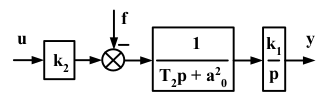
\includegraphics[width=0.5\linewidth]{pf.png}
		\caption{Объект управления}
		\label{fig:scr1}
	\end{figure}
	
	\section{Порядок выполнения работы}
	a) получение пмодели ВСВ
	
		Модель «Вход-состояние-выход» непрерывного объекта управления описывается уравнениями:
	\begin{equation}
	\begin{cases}
	\dot x(t) &= A x(t) + B u(t) + B_f f\\
	y(t) &= C x(t)
	\end{cases}
	\end{equation}
	С учетом заданных параметров в таблице 1, передаточная функция с рисунка 1 примент вид:
	\begin{equation}
		W(p) = \frac{k_1}{T_2 p + a_0^2} \frac{k_1}{p} =\frac{0.5}{0.95 p^2 + p} 
	\end{equation}

	Перейдем к канонической управляемой форме.

Для начала приведем передаточную функцию к виду с единичным старшим коэффициентом полинома.

\begin{equation}
W(p) = \frac{\frac{k_1 k_2}{T_2}}{p^2 + \frac{a_0^2}{T_2} p} = \frac{0.5263}{p^2 + 1.0526  p} 
\end{equation}

Теперь приведем к канонически управляемой форме:

\begin{equation}
A=
\begin{bmatrix}
0&1\\
0& -1.0526
\end{bmatrix}
\end{equation}
\begin{equation}
B=
\begin{bmatrix}
0\\
1
\end{bmatrix}
\end{equation}
\begin{equation}
C=
\begin{bmatrix}
0.5263&0
\end{bmatrix}
\end{equation}

Из рисунка 1 видно, что:
\begin{equation}
B_f=
\begin{bmatrix}
0\\
-1
\end{bmatrix}
\end{equation}

б) переход к дискретному описанию

Дискретная система описывается разностными уравнениями:
\begin{equation}
\begin{cases}
\dot x(k+1) &= A_d x(k) + B_d u(k) + B_{fd} f(k)\\
y(k) &= C x(k)
\end{cases}
\end{equation}

Для перехода к дискретной системе воспользуемся программой в Scilab.
	\begin{figure}[H]
	\center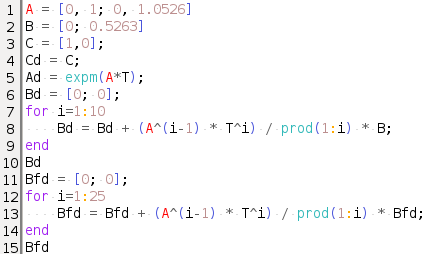
\includegraphics[width=0.5\linewidth]{pr.png}
	\caption{Программа рассчета дискретных матриц}
	\label{fig:scr1}
\end{figure}

Заданный в соответствии с вариантом интервал дискретности $T = 0.5$ сек.

В результате выполнения программы получим следующие матрицы:
\begin{equation}
A_d=
\begin{bmatrix}
    1&    0.3887642 \\ 
0&   0.5907868  
\end{bmatrix}
\end{equation}
\begin{equation}
B_d=
\begin{bmatrix}
    0.0556179  \\
0.2046066 \end{bmatrix}
\end{equation}
\begin{equation}
B_{fd} =
\begin{bmatrix}
  - 0.1056772 \\ 
- 0.3887642 \end{bmatrix}
\end{equation}

Матрица выходов системы не изменится:
\begin{equation}
C = C_d =
\begin{bmatrix}
1&0
\end{bmatrix}
\end{equation}


в) получение для дискретного входного воздействия модели ВСВ

Входное воздействие представлено линейной функцией:
\begin{equation}
	g(k) = g_0 = 4
\end{equation}
Следовательно
\begin{equation}
\xi_g(k) = g(k)
\end{equation}
\begin{equation}
\xi_g(k+1) = g(k+1) = g(k)
\end{equation}
Таким образом, матрицы модели входного воздействия принимают вид:
\begin{align}
	\Gamma_g = [1], H_g = [1]
\end{align}
Модель принимает вид:
\begin{equation}
	\begin{cases}
	\xi_g(k+1) &= \xi_g(k)\\
	g(k) &= \xi_g (k)
	\end{cases}
\end{equation}
Начальные условия: 
\begin{equation}
	\xi_g(0) = g0 = 4
\end{equation}
г) моделирование входного воздействия
\begin{figure}[H]
	\center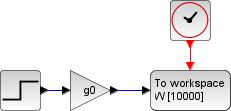
\includegraphics[width=0.4\linewidth]{gk.png}
	\caption{Схема моделирования входного воздействия}
	\label{fig:scr1}
\end{figure}
\begin{figure}[H]
	\center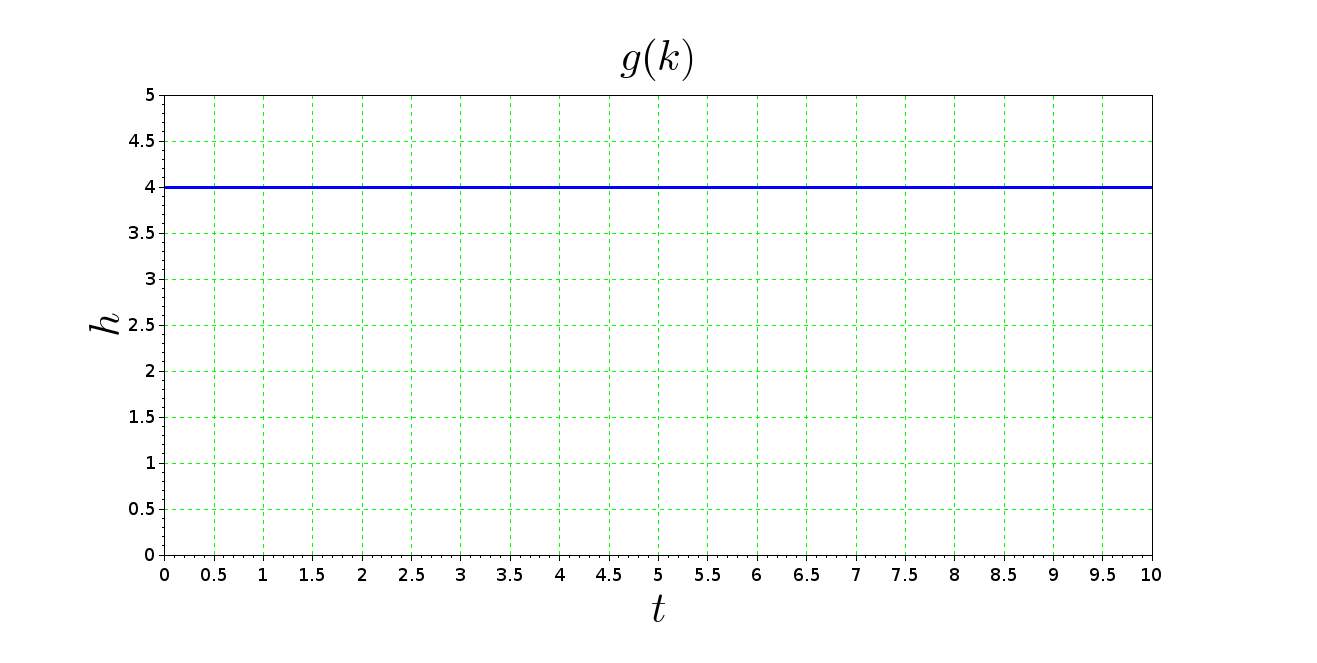
\includegraphics[width=0.7\linewidth]{gk_res.png}
	\caption{Результаты моделирования входного воздействия}
	\label{fig:scr1}
\end{figure}

д) вывод по полученной модели входного воздействия

Входное воздействие представлено пропорциональным звеном. Генерируемый сигнал соответствует модели.

e) синтез следящего алгоритма

Проверим систему на полную управляемость:

\begin{equation}
	det(U_d) = det
	\begin{bmatrix}
	0.0790224 &   0.3069223\\  
	0.3463289  &  0.5862164 
	\end{bmatrix}
	=
	 - 0.0599719 
\end{equation}

Так как матрица управляемости не вырождена, то система полностью управляема.

Проверим систему на полную наблюдаемость:

\begin{equation}
det(Q_d) = det
\begin{bmatrix}
1&    0\\         
1  &  0.6580447 
\end{bmatrix}
=
0.6580447  
\end{equation}

Так как матрица наблюдаемости не вырождена, то система является полностью наблюдаемой.

Чтобы построить оптимальную по быстродействию систему, необходимо назначить корни характеристического полинома следующим образом:

\begin{equation}
	z_i^* = 0
\end{equation}

Далее, из желаемых корней составим эталонную модель, для чего составим следующие матрицы:

\begin{equation}
\Gamma = 
\begin{bmatrix}
z^*_1 & 1 & 0\\
0 & z^*_2 & 1\\
0 & 0 & z^*_3
\end{bmatrix}
=
\begin{bmatrix}
0&1&0\\
0&0&1\\
0&0&0
\end{bmatrix}
\end{equation}
\begin{equation}
	H =
	\begin{bmatrix}
	1&0&0
	\end{bmatrix}
\end{equation}

Введем уравнения движения расширенного объекта, присоединив уравнение регулятора:
\begin{equation}
	\begin{cases}
	v(k+1) = v(k) + g(k) - x_1 (k)\\
	x(k+1) = A_d x(k) + B_d u(k)
	\end{cases}
\end{equation}

Представим расширенный вектор состояния:
\begin{equation}
	\bar x = 
	\begin{bmatrix}
	v\\
	x
	\end{bmatrix}
\end{equation}

Рассчитаем матрицы:
\begin{equation}
	\bar A_d =
	\begin{bmatrix}
	1 & -C_d\\
	0 & A_d
	\end{bmatrix}
=
\begin{bmatrix}
    1& - 1&    0\\        
0&   1&   0.3887642  \\
0&   0&    0.5907868 
\end{bmatrix}
\end{equation}
\begin{equation}
\bar B_d =
\begin{bmatrix}
0\\
B_d
\end{bmatrix}
=
\begin{bmatrix}
0\\
    0.0556179  \\
0.2046066 
\end{bmatrix}
\end{equation}

Расширенная система примет вид:

\begin{equation}
	\begin{cases}
	\bar x(k+1) = \bar A_d \bar x(k) + \bar B_d u(k) + B_g g(k) \\
	u(k) = k_g g - \bar k_d \bar x(k)
	\end{cases}
\end{equation}
\begin{equation}
	\bar x(k+1) = (\bar A_d - \bar B_d \bar k_d) \bar x (k) +  (k_g \bar B_d + B_g) g(k)
\end{equation}

Теперь вычислим МЛСОС из системы с матричным уравнением типа Сильвестра.

\begin{equation}
	\begin{cases}
	M \Gamma - \bar A_d M = \bar B_d H\\
	K_d = - H M^{-1}
	\end{cases}
\end{equation}

Расчет матрицы $K_d$ произведем в среде моделирования $Scilab$:

\begin{align}
	M &= sylv(-A_d,\Gamma, B_d * H, 'd');\\
	Kd &= -H * M^{-1};
\end{align} 

\begin{equation}
K_d = 
	\begin{bmatrix}
k_1 &   k_2 & k_3   
\end{bmatrix}=
	\begin{bmatrix}
	      - 9.7748568  &  24.010399 &   6.1355721    
	\end{bmatrix}
\end{equation}

ж) моделирование

\begin{figure}[H]
	\center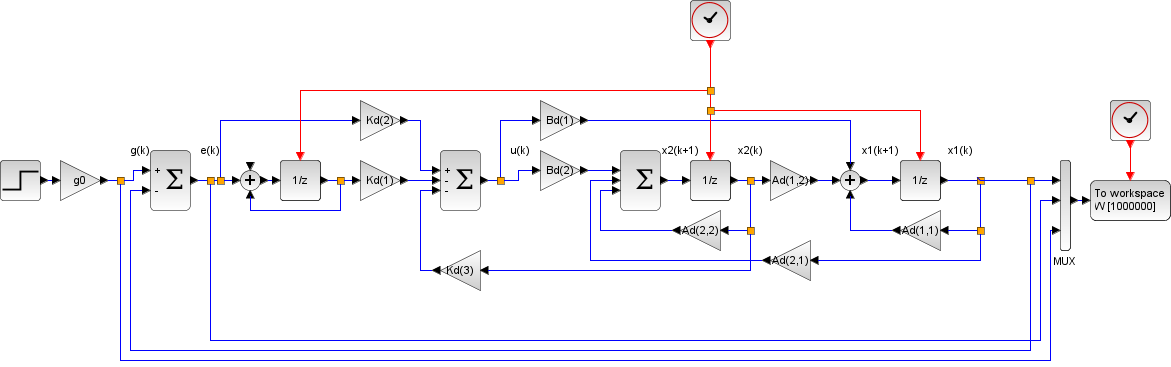
\includegraphics[width=1\linewidth]{model_sch.png}
	\caption{Схема моделирования}
	\label{fig:scr1}
\end{figure}
\begin{figure}[H]
	\center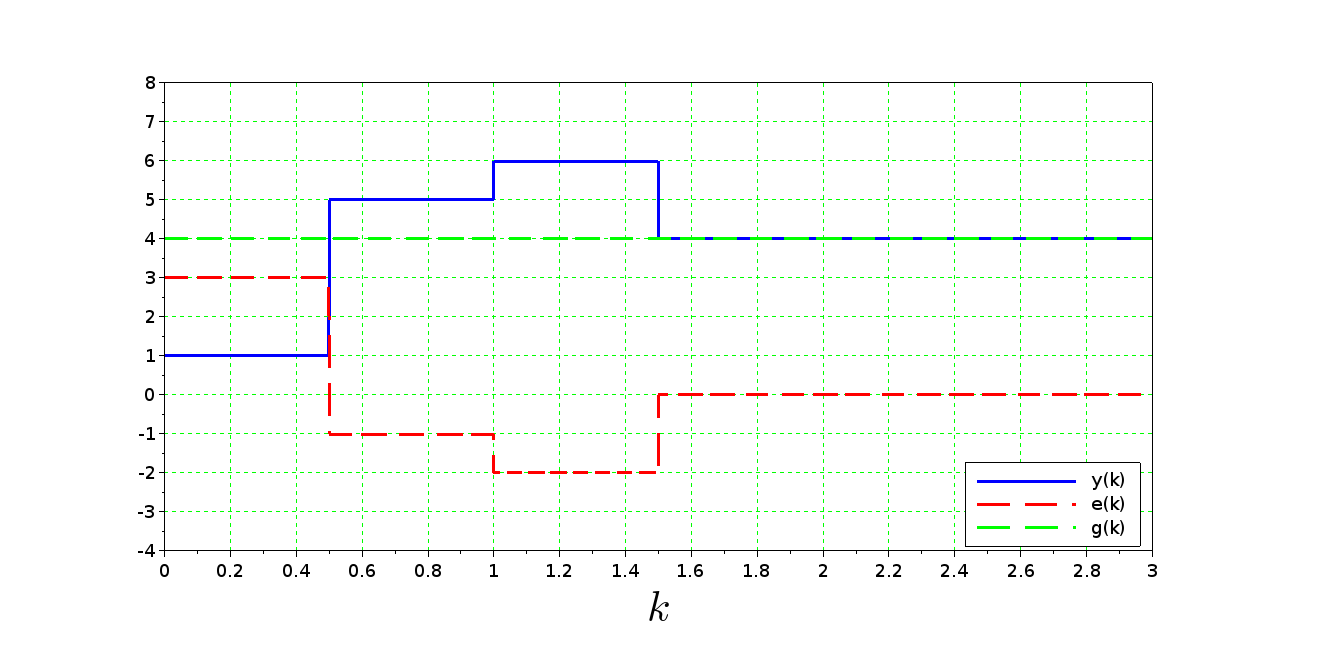
\includegraphics[width=1\linewidth]{model_res.png}
	\caption{Результаты моделирования }
	\label{fig:scr1}
\end{figure}

з) вывод по модели

Как видно из графиков на рисунке 6, синтезированный регулятор справляется с
задачей слежения за задающим сигналом  $g(k)$ достаточно хорошо, обеспечивая
нулевую ошибку $e(k)$.

и) модель возмущающего воздействия

Согласно варианту:

\begin{eqnarray}
f_0 = 3.26\\
f_1 = 3.95\\
T = 0.5
\end{eqnarray}

Таким образом, возмущающее воздействие представляет собой линейно-нарастающую функцию:
\begin{equation}
	g(k) = f_0 + f_1 k T = 3.26 + 1.975 k
\end{equation}

Представим возмущающее воздействие в виде модели в пространстве состояний:

\begin{equation}
\begin{cases}
	\xi_g (k+1) &= \Gamma_g \xi(k)\\
	g(k) &= H_g \xi (k)
\end{cases}
\end{equation}

Найдем переменные состояния:
\begin{eqnarray}
&g(k) = 3.26 + 1.975 k \\
&\xi (k) = g(k)\\
&\xi (k+1) = 3.26 + 1.975 k + 1.975 = \xi (k) + 1.975
\end{eqnarray}

Отсюда, найдем матрицы:
\begin{eqnarray}
	\Gamma_g &= [1]\\
	H_g &= [1]
\end{eqnarray}

Модель примет вид:

\begin{equation}
\begin{cases}
\xi_g (k+1) &= \xi(k) + 1.975\\
g(k) &= \xi (k)
\end{cases}
\end{equation}

Начальные условия, при $k = 0$:

\begin{equation}
	\xi (0) = 3.26
\end{equation}

На основе полученной модели и начальных условий, произведем моделирование.

к) моделирование возмущающего воздействия


\begin{figure}[H]
	\center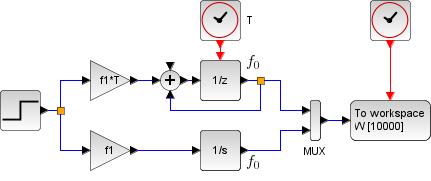
\includegraphics[width=0.7\linewidth]{input_fsch.png}
	\caption{Схема моделирования}
	\label{fig:scr1}
\end{figure}
\begin{figure}[H]
	\center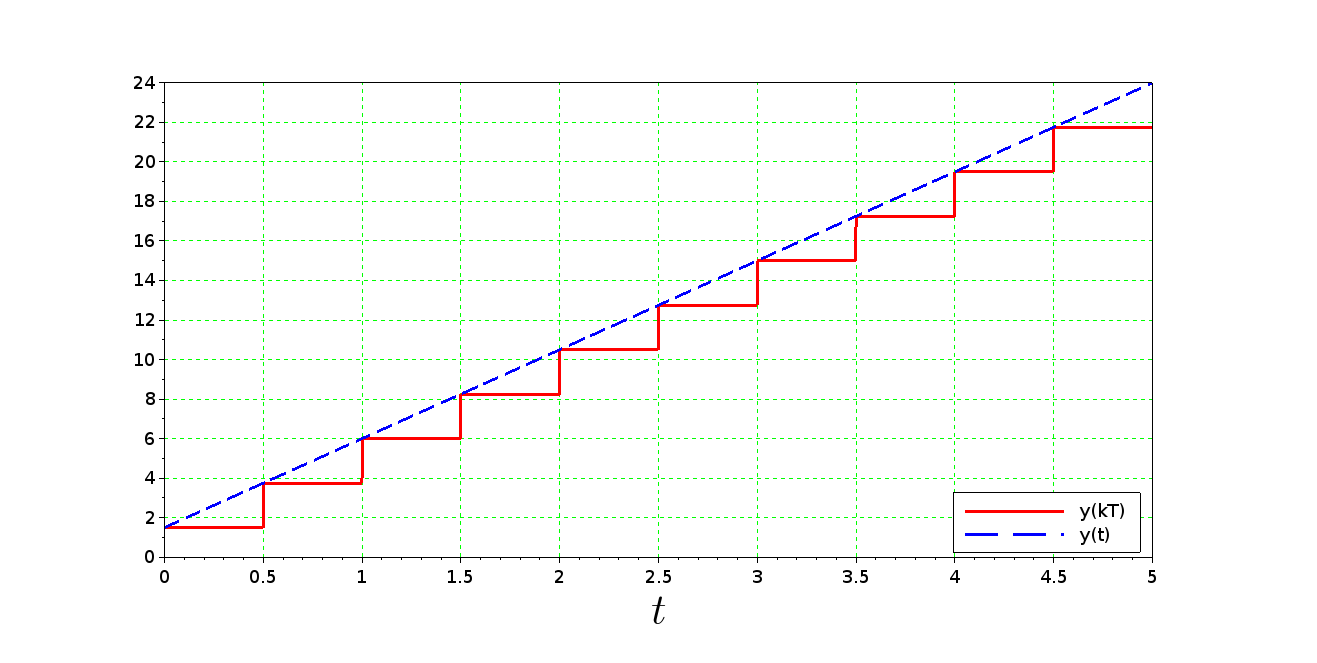
\includegraphics[width=1\linewidth]{input_f.png}
	\caption{Результаты моделирования }
	\label{fig:scr1}
\end{figure}

Непрерывный задающий сигнал был получен методом последовательного дифференцирования:

\begin{eqnarray}
	&g(t) = 3.26 + 3.95t\\
	&\dot g(t) = 3.95\\
	&g(0) = 3.26
\end{eqnarray}

л) анализ полученной модели

Как видно из рисунка 8, полученная дискретная модель точносоответствует модели, генерирующей непрерывный аналог сигнала вида.  Следовательно, можно сделать вывод о состоятельности модели.

м) Синтез алгоритмов управления, обеспечивающих нулевую установившуюся ошибку замкнутой системы при наличии возмущений

В случае наличия возмущающих воздействий, в регуляторе появляется соответствующая прямая связь и управляющее воздействие определяется уравнением:

\begin{equation}
	u(k)= k_1 g(k)  - \overline{k} \overline{x} (k) - k_f x_f  (k)
\end{equation}

где $k_f$ -- матрица линейных прямых связей от возмущающего воздействия, $x_f ( k )$ -- вектор состояния возмущающего воздействия.

Матрицу $k_f$ найдем из уравнения:

\begin{equation}
	B_d k_f = B_{fd} H_f
\end{equation}
\begin{equation}
	\begin{bmatrix}
    0.0556179   * k_{f1} \\
0.2046066  * k_{f1} 
	\end{bmatrix}
	=
	\begin{bmatrix}
	 - 0.1056772 \\ 
	- 0.3887642  
	\end{bmatrix}
\end{equation}

откуда

\begin{equation}
	k_f = 
	\begin{bmatrix}
	-1.9 & 0
	\end{bmatrix}
\end{equation}

н) Моделирование замкнутой системы при наличии возмущающего воздействия

\begin{figure}[H]
	\center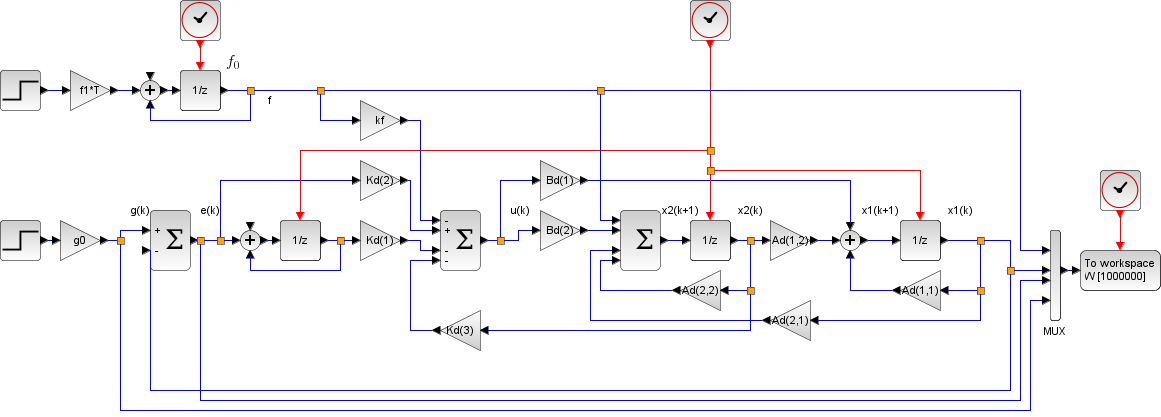
\includegraphics[width=1	\linewidth]{model_f.png}
	\caption{Схема моделирования}	
	\label{fig:scr1}
\end{figure}
\begin{figure}[H]
	\center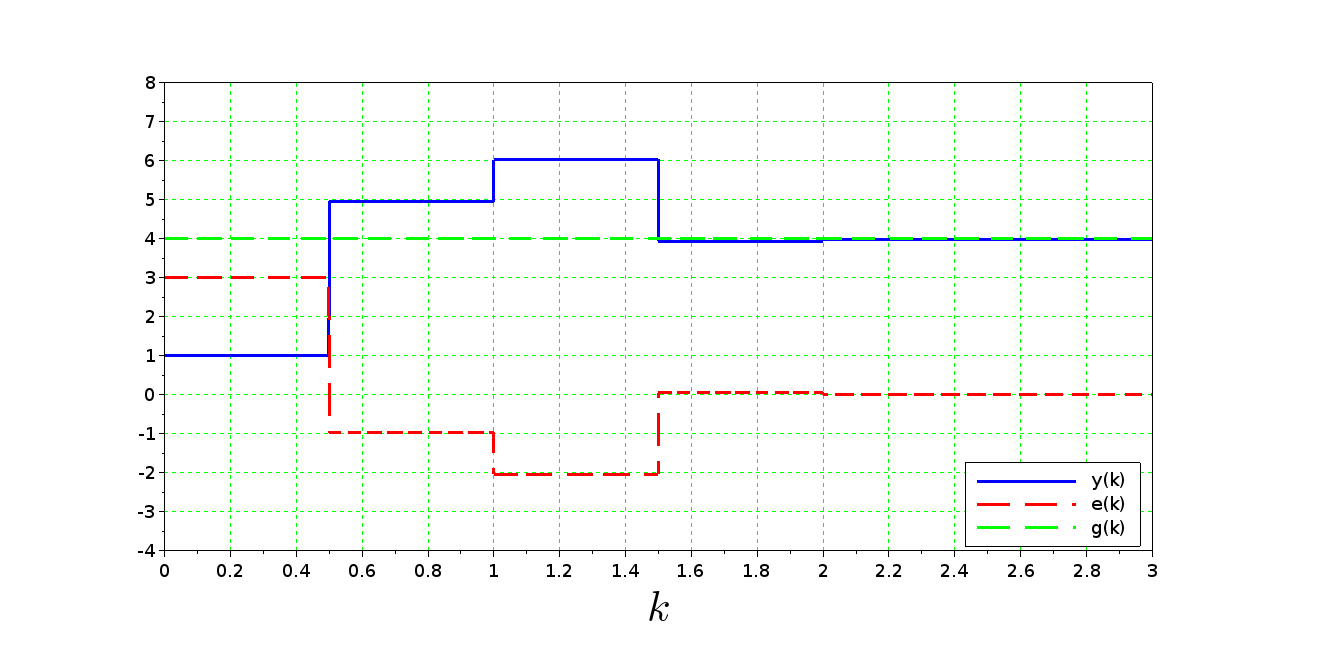
\includegraphics[width=1\linewidth]{model_f_res.png}
	\caption{Результаты моделирования }
	\label{fig:scr1}
\end{figure}

о) анализ результатов моделирования

Рисунок 10 показывает, что несмотря на возмущения, регулятор справляется со своей задачей и сводит ошибку к нулю

\subsection{Заключение}

В ходе работы были освоены принципы синтезирования дискретных
регуляторов для систем слежения. С задачей слежения за линейным сигалом великолепно справляется интегральный регулятор, сводящий ошибку слежения в ноль даже в случае присутствия возмущающий воздействий.

\end{document}

